\documentclass[a4paper]{article}

\usepackage[english]{babel}
\usepackage[utf8]{inputenc}
\usepackage[color=blue!20]{todonotes}
\usepackage{titlesec}

\newcommand{\itab}[1]{\hspace{0em}\rlap{#1}}
\newcommand{\tab}[1]{\hspace{.2\textwidth}\rlap{#1}}
\usepackage{hyperref}
\usepackage{float}

\usepackage{listings}

\lstdefinelanguage{nagconf}
  {
  frame=tb,
  aboveskip=3mm,
  belowskip=3mm,
  showstringspaces=false,
  columns=flexible,
  basicstyle={\small\ttfamily},
  numbers=none,
  breaklines=true,
  breakatwhitespace=true
  tabsize=3
  }

\title{The Merits of Using Ansible and Nagios Together}

\author{Michael Pobega (pobegam@sunyit.edu)}

\date{\today}

\begin{document}
\begin{titlepage}
\clearpage\maketitle
\thispagestyle{empty}

\begin{abstract}
Overview of the use of Nagios and Ansible on the same machine and/or network, and how they can complement each other.
\end{abstract}

\clearpage
\thispagestyle{empty}
\tableofcontents
\end{titlepage}
\clearpage

\section{Nagios Retrospective}

\subsection{Deployment}

This was the most daunting part of my entire Capstone. Deploying Nagios was a complete pain; a majority of the work was information gathering and firewall modifications.

\begin{figure}[H]
\centering
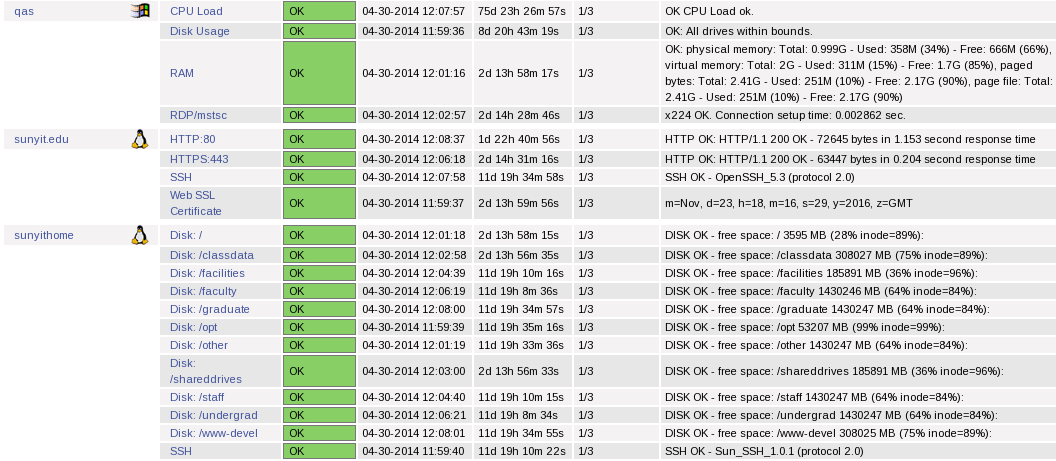
\includegraphics[width=0.9\textwidth]{nagios-services.png}
\caption{\label{fig:nagserv}Nagios listing of hosts and services.}
\end{figure}

The first servers added were added from a list obtained from an old Nagios server, but the rest had to be gathered by hand. After weeks in VCenter gathering system information including hostnames, IPs, and services, the Nagios server was finally ready to be deployed. 

Hostgroups were created to easily manage batch commands for multiple hosts. These hostgroups include Linux, Windows, NRPE, NSClient++, Webservers and MySQL Cluster (which as of the time of writing was still being used, but is now deprecated).

\subsection{Security}

The server sits behind a firewall and is only accessible from the administrative subnet. There isn't much else to say about this, limiting access seems to be the best practice for securing a Nagios server.

\subsection{Conclusion}

This is a simple server and I don't have too much to say about it that hasn't already been said better by someone else. The majority of the work for this server was busy work, and besides keeping watch on Apache and Linux exploits the server is secured via firewall making it inaccessible by the outside world.

\begin{figure}[H]
\centering
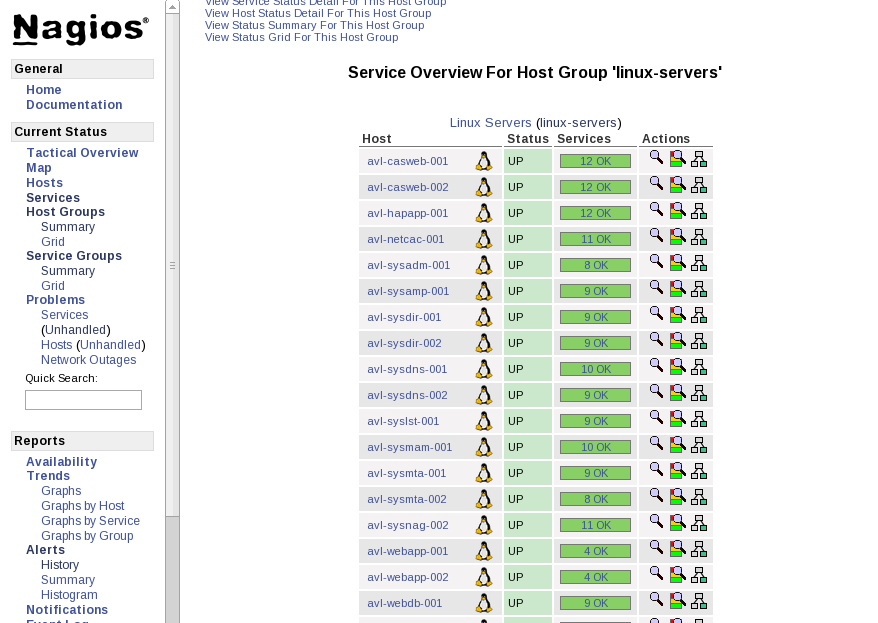
\includegraphics[width=0.9\textwidth]{nagios-linux.png}
\caption{\label{fig:naglin}Linux hostgroup view inside of Nagios.}
\end{figure}

\section{Ansible Retrospective}

\subsection{Deployment}
Deployment of Ansible on a network is near trivial. Because Ansible uses SSH as it's connection method it doesn't require any additional software installed on any of the clients, meaning deployment is as simple as \textit{`yum install ansible'}. This is probably Ansible's biggest strength over other equally (or even moreso) robust solutions such as Puppet, Chef and Salt. 

The client nodes need to have the ansible account present and accessible via SSH. The solution I've deployed uses SSH keys to connect and the local ansible accounts have randomized passwords (just to lower the possible attack vectors by one). Currently the template used to create new VMs has the Ansible account already present, but for any legacy machines that don't have the account already it can be created easily; just add an ansible user/group and copy the public SSH key.

\subsection{Security}
Initially in my first draft of this paper this paragraph talked about how it was great that Ansible uses standardized packages such as OpenSSH and OpenSSL to handle it's connection and encryption, but it's since been rewritten in response to the Heartbleed Bug.

Using standard libraries and packages such as OpenSSH and OpenSSL offer huge security benefits; they get patched constantly by upstream/disto maintainers, they are guaranteed to be thoroughly tested, and come standard with most *nix systems. The other side of the coin, however, is that they are also bigger targets. Bugs and exploits may very well exist and not be publicized, such as the Heartbleed vulnerability that existed in the OpenSSL code for two years (an eternity in terms of security).

Another big portion of security has to do with how accessible the administrator wants the servers to be. On the one hand, the ansible account can be setup to have full sudo access with NOPASSWD on every system; this allows password-less use of the \textit{--sudo} flag when calling Ansible. On the other hand if the \textit{ansible} user account is ever cracked or broken in to the user will have full root access to the system, which could quickly turn into a network-wide problem if the hacker is crafty enough.

One way around this is to only enable the ansible account to have NOPASSWD access to specific binaries on the system. The issue with this approach is that each server's \textit{sudoers} file would have to be modified by hand to add or remove permissions, which could end up being a huge undertaking.

\begin{lstlisting}[language=nagconf]
ansible ALL=NOPASSWD: /sbin/shutdown, /sbin/reboot, /usr/bin/yum
\end{lstlisting}
\hfill \textit{/etc/sudoers: limited permissions}\\

Another workaround is to specify the root passwords at runtime when calling Ansible, but this is time consuming if all of the servers have different passwords.

All in all, Ansible is a very secure choice for automation. Gaining access to the Ansible server doesn't automatically give access to the nodes due to it's use of SSH host keys, unlike other automation suites such as Salt, where breaking into the master would encompass a full network compromise. On the topic of Salt it uses it's own AES implementation which has been proven in the past to not be the most secure implementation; another +1 for using standard SSH as a transport.

\subsection{Everyday Use (and misuse)}

In my time playing with Ansible I've used it to automate a lot of things; I've also made some rookie mistakes in the process of learning Ansible.

Originally I didn't realize how powerful Ansible modules are or that Ansible could iterate over commands, and had HUGE playbooks of one line commands (which I won't include for the reader's sanity). \textit{ansible-doc} has become my go-to command for the past few months even moreso than \textit{man}; you can find documentation for all of the Ansible modules listed there, which makes writing one-liners or code during an internet outage a breeze. 

By the way, Ansible iteration looks like this:
\begin{lstlisting}[language=nagconf]
    - name: yum update stuff (this step takes a while)
      yum: name={{ item }} state=latest
      with_items:
       - openssl
       - openssl-devel
       - rng-tools
       - keepalived
\end{lstlisting}
\hfill \textit{Iteration/multiple arguments in an Ansible Playbook}\\

\begin{figure}[H]
\centering
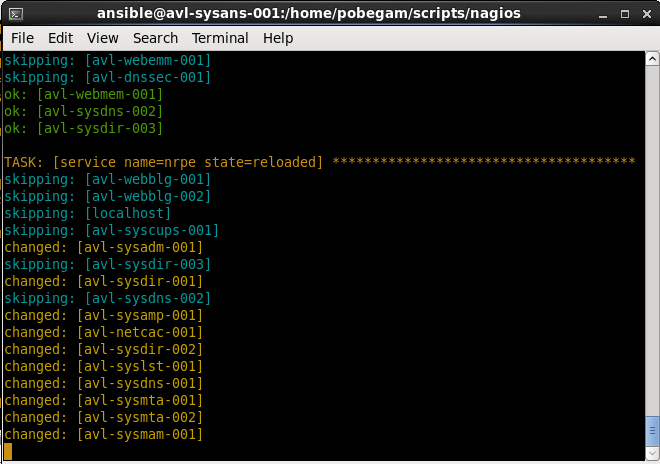
\includegraphics[width=0.9\textwidth]{ansible-in-action.png}
\caption{\label{fig:ansinact}Ansible doing it's thing.}
\end{figure}

I've used Ansible for multiple things (which I will list but are documented elsewhere):
\begin{itemize}
	\item DNSSEC Deployment for sunyct.edu
    \item Deploying DNS failover
    \item Distributing and enabling scripts and cronjobs to enable functionality between servers and ServiceDesk
    \item Enabling remote syslogging
    \item Deploying memcache for a Wordpress server
    \item Installing NRPE (both from yum and from source at separate times) on multiple servers
    \item Distributing and updating custom commands and scripts for servers monitored by NRPE
\end{itemize}

Ansible has also been invoked on the command line manually to do multiple things, such as scan for and patch known Linux exploits/rootkits, including Heartbleed and the recent \_\_UMBREON\_\_ rootkit.

\subsection{Conclusion}

Ansible is a FANTASTIC tool that I will be using in the future. It has taught me a lot about automation and the mindset involved, and it's given me a great toolset to bring with me into the world of Sysadmin'ing.

\section{Ansible and Nagios}

Ansible and Nagios are two tools with a very Unixy mindset; they each do one thing and they do it well, while relying on other tools to fill in the blanks. Nagios monitors and alerts and does those tasks amazingly well, but automating anything requires a separate tool; in this case, Ansible.

\begin{figure}[H]
\centering
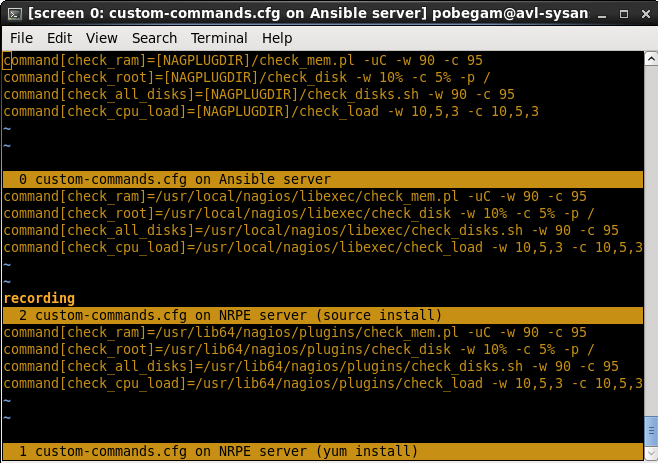
\includegraphics[width=0.9\textwidth]{customcommands.png}
\caption{\label{fig:customcommands}custom-commands.png on three different servers}
\end{figure}

Ansible was used to deploy and administer the servers that Nagios monitored. NRPE installs were automated and can now be rapidly redeployed, while NSClient++ (Windows' NRPE) must be installed manually on each server, which has proven to be a time consuming task.

Another issue we ran into was using arguments with NRPE. Our legacy servers have NRPE installed with arguments disabled at compile time, so using NRPE arguments is out of the question. This means that commands must be statically defined in a local file on each server. Ansible makes updating these files (and uploading the shell scripts that are run) very simple -- it's just a matter of identifying the folders the files need to be put into and copying them.

Ansible solved all of these issues in a very elegant fashion. It checks what kind of server it is dealing with:

\begin{lstlisting}[language=nagconf]
    - name: check if /etc/nrpe.d/ exists
      stat: path=/etc/nrpe.d/
      register: nrpe_exists
    - name: check if /etc/init.d/nrpe exists
      stat: path=/etc/init.d/nrpe
      register: nrpe_initd
    - name: check if /etc/xinetd.d/nrpe exists
      stat: path=/etc/xinetd.d/nrpe
      register: nrpe_xinetd
\end{lstlisting}
\hfill \textit{Discovering information about NRPE servers}\\

Then it copies the file to the proper directory based on the previous tests:

\begin{lstlisting}[language=nagconf]
    - name: Uploading $REMOTE$:/etc/nrpe.d/custom-commands.cfg for yum install
      copy: src=/srv/nfs/nrpe/custom-commands.cfg dest=/etc/nrpe.d/custom-commands.cfg owner=nrpe group=nrpe mode=750 force=yes
      when: nrpe_exists.stat.exists and nrpe_initd.stat.exists
    - name: Uploading $REMOTE$:/etc/nrpe.d/custom-commands.cfg for src install
      copy: src=/srv/nfs/nrpe/custom-commands.cfg dest=/etc/nrpe.d/custom-commands.cfg owner=nagios group=nagios mode=750 force=yes
      when: nrpe_exists.stat.exists and nrpe_xinetd.stat.exists
\end{lstlisting}
\hfill \textit{Copying files to NRPE servers}\\

And uses sed to replace the text \textit{[NAGPLUGDIR]} with the proper directory for that system.

\begin{lstlisting}[language=nagconf]
    - name: Updating $REMOTE$:/etc/nrpe.d/custom-commands.cfg for yum install
      command: sed -i "s#\[NAGPLUGDIR\]#/usr/lib64/nagios/plugins#g" /etc/nrpe.d/custom-commands.cfg
      when: nrpe_exists.stat.exists and nrpe_initd.stat.exists
    - name: Updating $REMOTE$:/etc/nrpe.d/custom-commands.cfg for src install
      command: sed -i "s#\[NAGPLUGDIR\]#/usr/local/nagios/libexec#g" /etc/nrpe.d/custom-commands.cfg
      when: nrpe_exists.stat.exists and nrpe_xinetd.stat.exists
\end{lstlisting}
\hfill \textit{Modifying custom-commands.cfg}\\

Then it copies over all of the custom scripts from the Ansible server and places them into the Nagios plugin directory, and finally restarts the daemon (nrpe or xinetd based on the install method):

\begin{lstlisting}[language=nagconf]
    - name: Copy over custom NRPE executables for yum install
      copy: src=/srv/nfs/nrpe/libexec/ dest=/usr/lib64/nagios/plugins/ owner=nrpe group=nrpe mode=750
      when: nrpe_exists.stat.exists and nrpe_initd.stat.exists
    - name: Copy over custom NRPE executables for src install
      copy: src=/srv/nfs/nrpe/libexec/ dest=/usr/local/nagios/libexec/ owner=nagios group=nagios mode=750
      when: nrpe_exists.stat.exists and nrpe_xinetd.stat.exists

    - service: name=nrpe state=reloaded
      when: nrpe_initd.stat.exists
    - service: name=xinetd state=reloaded
      when: nrpe_xinetd.stat.exists
\end{lstlisting}
\hfill \textit{Modifying and copying the rest of the files for NRPE}\\

This playbook has completely trivialized NRPE deployment. Initially, when I wanted to create a new command or modify a previously existing one I had to do it server by server. After Ansible, though, the process is as simple as creating the script on the Ansible server, running the Playbook, and modifying the relevant hosts/hostgroups in Nagios.

Keep in mind this playbook only represents one use of Ansible and Nagios in conjunction; Anything Nagios needs that requires changes on the client side would be wholly trivialized with Ansible.

Between this, the simplified NRPE deployment and all of the one liners used to manage groups of servers simultaneously, Ansible has proven itself to be a completely irreplacable tool when used in conjuction with Nagios. It fills a lot of the voids that Nagios doesn't (by definition Nagios is only a monitoring tool), and allows an administrator to make sweeping changes to monitored hosts with one simple command.

\end{document}